\chapter{Experimental Setup}\label{Chapter:experiments}


\section{Lookup Tables} \label{exp:lt}

\subsection{AG Trace}
As explained in section \ref{pm:ag-ponder} attentive guidance can help in mocking the pondering. For a lookup table composition of the form \lq $((000)t3)t1$ AG enforces pondering as follows:
\begin{equation}
t1(111) = 100 \qquad t3(000) = 111 \qquad ((000)t3)t1 = 100,
\end{equation}
the composed function is expanded as follows:
\begin{equation}
000\ t3\ t1 = 000\ 111\ 100.
\end{equation}
AG therefore forces the decoder to ponder for two additional steps. The biggest difference from the Pondering in section \ref{mtv:ponder} would be that at each pondering step we have an emission, instead of the ponder step being a silent one. The trace for the attentive guidance can be explained as follows and is shown in figure \ref{ag_lt}:
\begin{itemize}
	\item The first step is the copy step where the three bit input to the composition is copies as if.
	\item After this the tables in the composition are applied sequentially to the three bit input preceding them.
	\item The diagonal trace is mean to capture this sequential and compositional solution of lookup tables. At each step of decoding we force the model to focus on only that input prompt which results in the correct output for that step.
\end{itemize}


\subsection{Accuracy}
Since the lookup tables can be viewed as nested functions, accuracy of final output of the composition can be an adequate measure of model performance. However since we want to ensure that the model doesn't learn spurious patterns in data to land at an un-compositional solution, we want it to be accurate at each step of the composition. This hierarchical measure of accuracy is a viable test for the compositionality of the network. Therefore in all evaluations \textit{sequence accuracy} is the performance metric of the model.

\subparagraph{Hyperparameters}: Based on the hyperparameter grid search conducted by \cite{Hupkes2018} I ran the experiments with the best hyperparameters for both baseline (RNN cell=GRU, Embedding size=128, Hidden layer size=512, optimizer=Adam \citep{KingmaB14}, learning rate=0.001, attention=pre-rnn \citep{Bahdanau2014}, alignment measure=mlp(section \ref{mtv:attn})).

\section{Symbol Rewriting} \label{exp:sr}

\begin{figure}[ht] 
	\begin{subfigure}[b]{0.5\linewidth}
		\centering
		\ifpdf
		\includegraphics[width=0.95\linewidth]{./figs/lookup/lt-trace-pdf}
		\else
		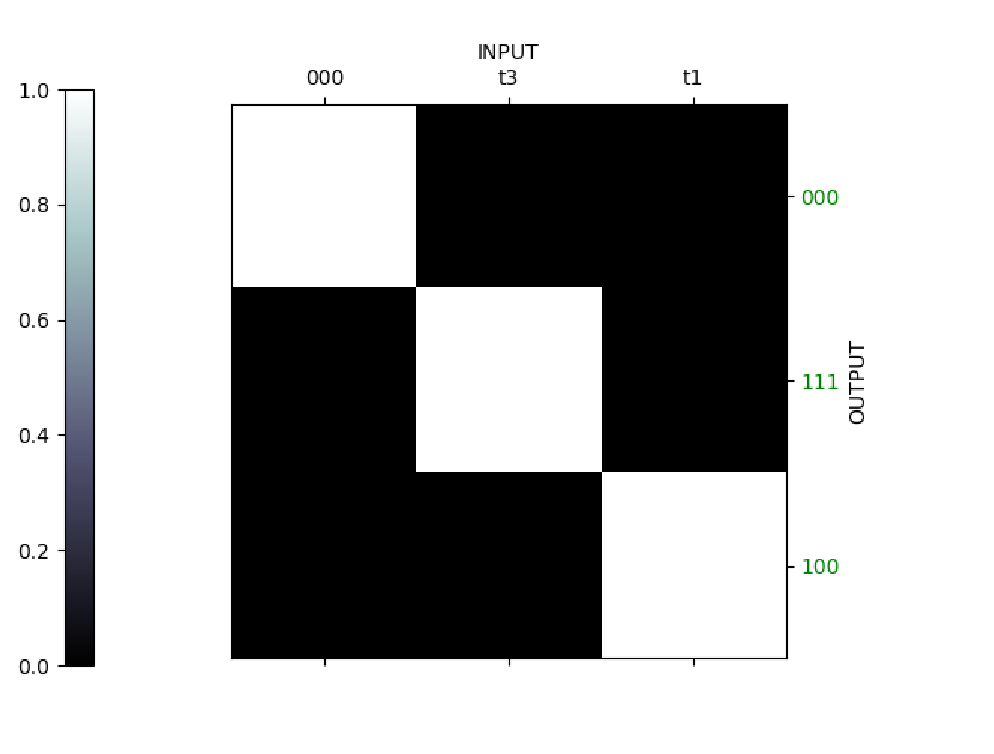
\includegraphics[width=0.95\linewidth]{./figs/lookup/lt-trace-eps}
		\fi
		\caption{AG Trace for Lookup Tables} 
		\label{ag_lt} 
		\vspace{2ex}
	\end{subfigure}%% 
	\begin{subfigure}[b]{0.5\linewidth}
		\centering
		\ifpdf
		\includegraphics[width=0.95\linewidth]{./figs/lookup/sr-trace-pdf}
		\else
		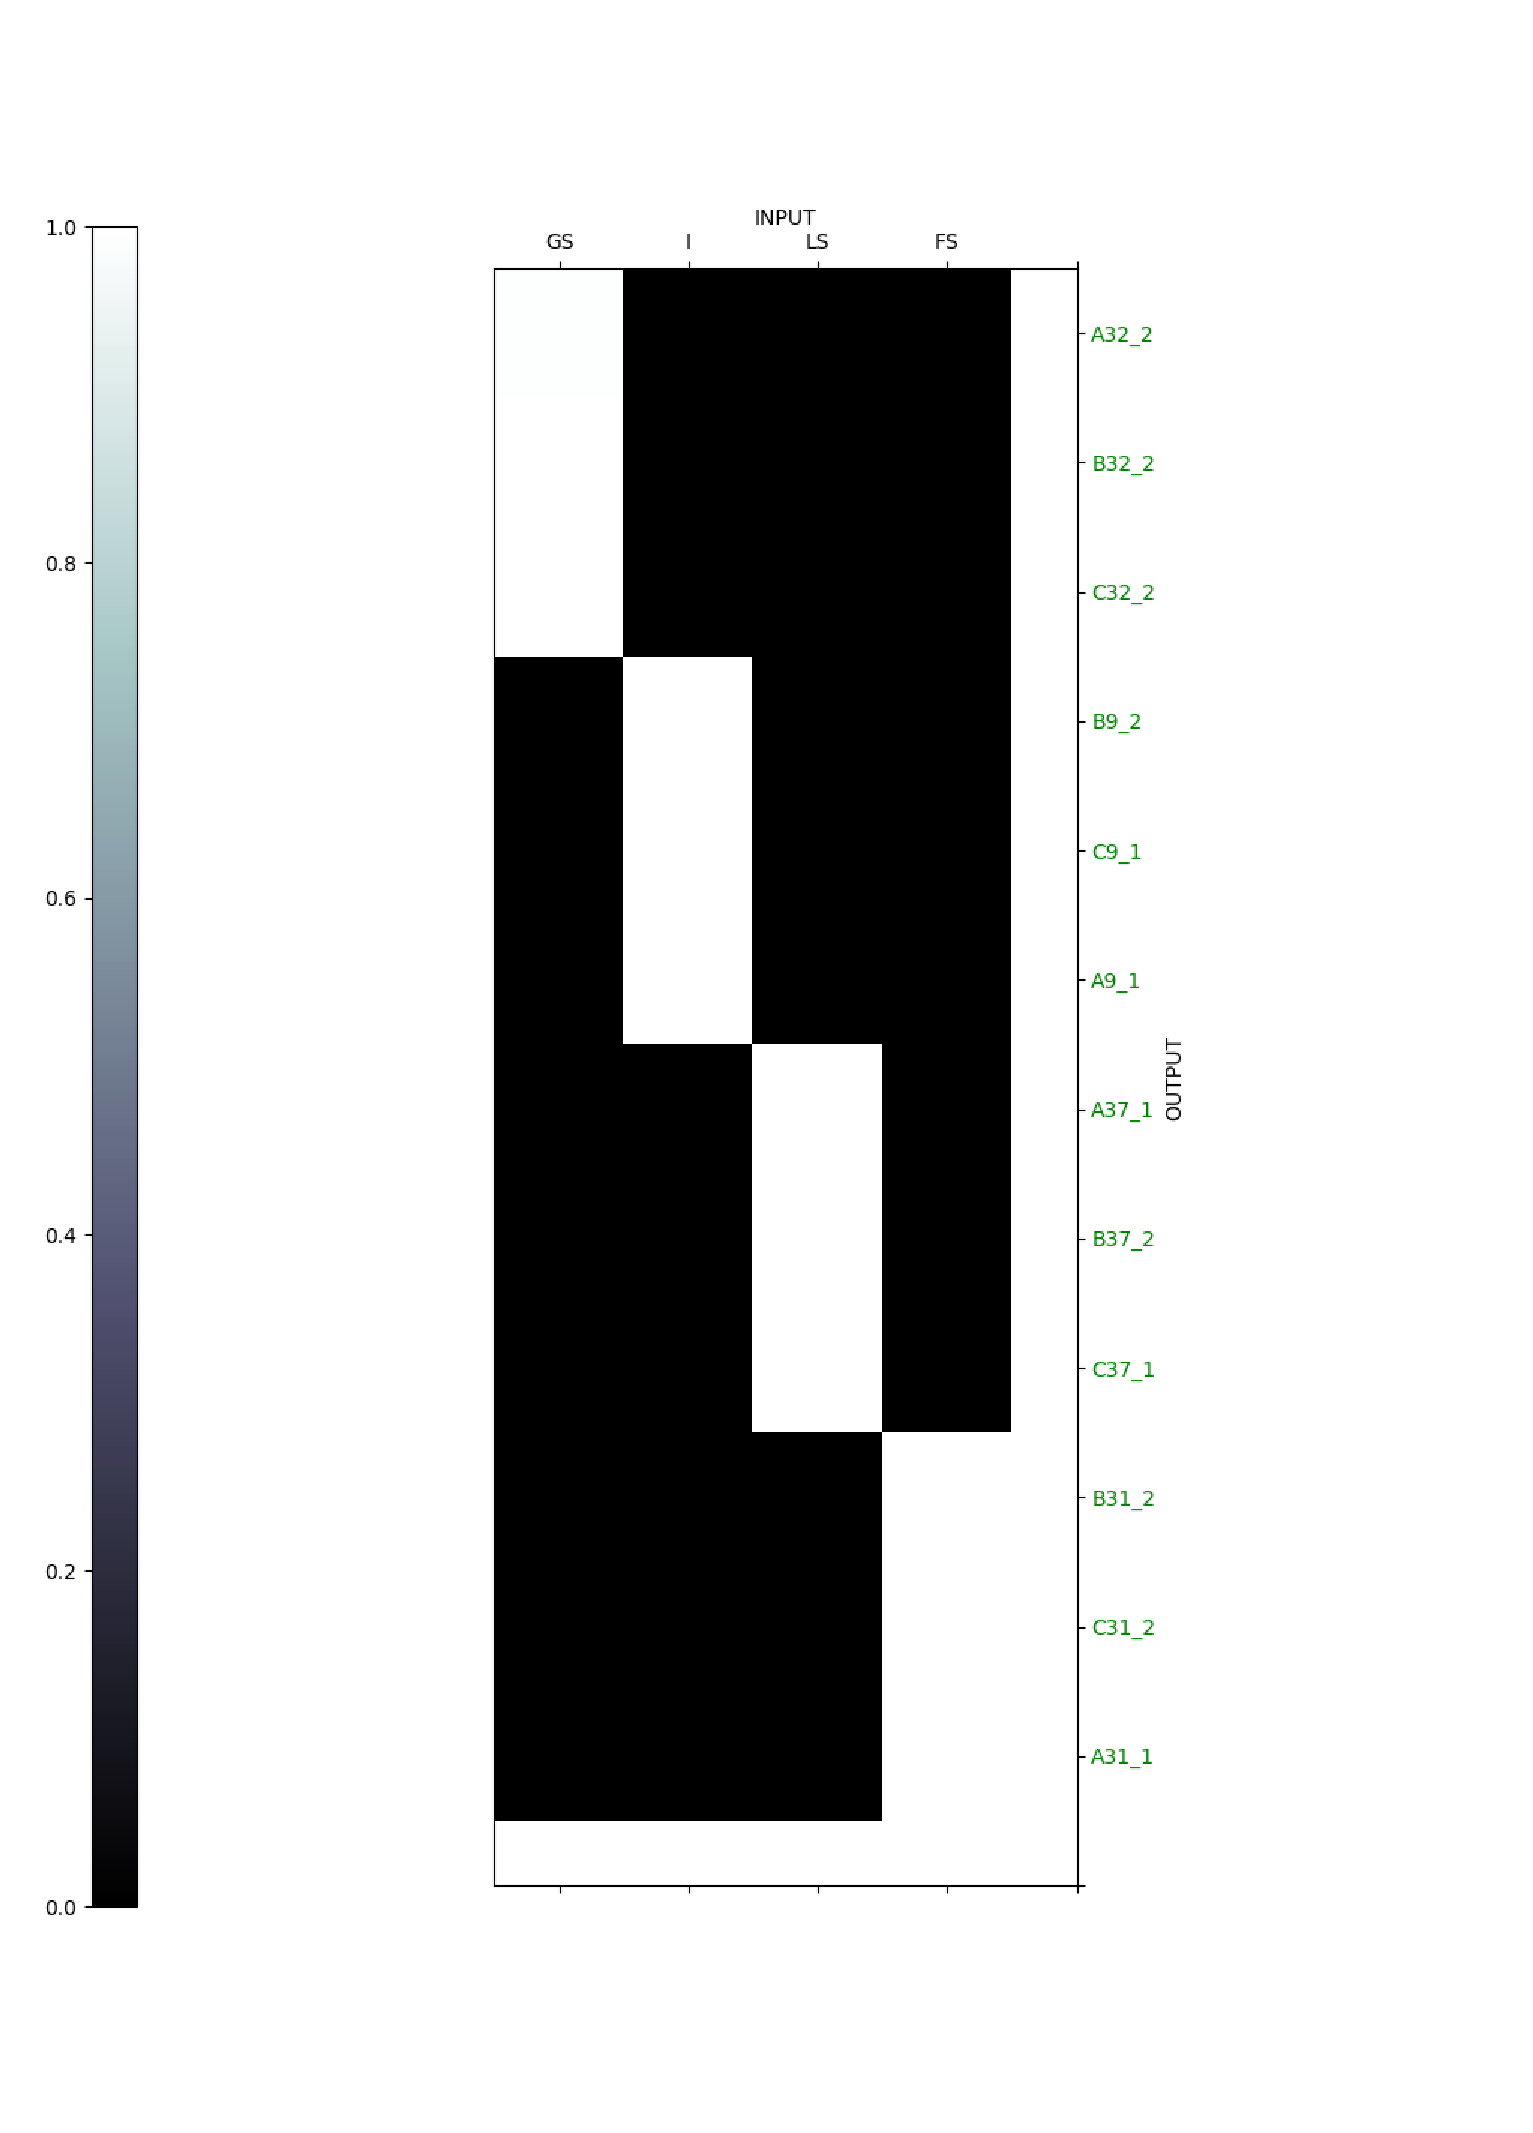
\includegraphics[width=0.95\linewidth]{./figs/lookup/sr-trace-eps}
		\fi 
		\caption{AG Trace for Symbol rewriting} 
		\label{ag_sr} 
		\vspace{2ex}
	\end{subfigure}
	\caption{Attentive Guidance Trace for Lookup tables and Symbol rewriting tasks}
	\label{lt_sr_trace}
\end{figure}